% Options for packages loaded elsewhere
\PassOptionsToPackage{unicode}{hyperref}
\PassOptionsToPackage{hyphens}{url}
%
\documentclass[
]{article}
\usepackage{lmodern}
\usepackage{amssymb,amsmath}
\usepackage{ifxetex,ifluatex}
\ifnum 0\ifxetex 1\fi\ifluatex 1\fi=0 % if pdftex
  \usepackage[T1]{fontenc}
  \usepackage[utf8]{inputenc}
  \usepackage{textcomp} % provide euro and other symbols
\else % if luatex or xetex
  \usepackage{unicode-math}
  \defaultfontfeatures{Scale=MatchLowercase}
  \defaultfontfeatures[\rmfamily]{Ligatures=TeX,Scale=1}
\fi
% Use upquote if available, for straight quotes in verbatim environments
\IfFileExists{upquote.sty}{\usepackage{upquote}}{}
\IfFileExists{microtype.sty}{% use microtype if available
  \usepackage[]{microtype}
  \UseMicrotypeSet[protrusion]{basicmath} % disable protrusion for tt fonts
}{}
\makeatletter
\@ifundefined{KOMAClassName}{% if non-KOMA class
  \IfFileExists{parskip.sty}{%
    \usepackage{parskip}
  }{% else
    \setlength{\parindent}{0pt}
    \setlength{\parskip}{6pt plus 2pt minus 1pt}}
}{% if KOMA class
  \KOMAoptions{parskip=half}}
\makeatother
\usepackage{xcolor}
\IfFileExists{xurl.sty}{\usepackage{xurl}}{} % add URL line breaks if available
\IfFileExists{bookmark.sty}{\usepackage{bookmark}}{\usepackage{hyperref}}
\hypersetup{
  pdftitle={03 Data Analysis},
  pdfauthor={Thomas J. Brailey},
  hidelinks,
  pdfcreator={LaTeX via pandoc}}
\urlstyle{same} % disable monospaced font for URLs
\usepackage[margin=1in]{geometry}
\usepackage{color}
\usepackage{fancyvrb}
\newcommand{\VerbBar}{|}
\newcommand{\VERB}{\Verb[commandchars=\\\{\}]}
\DefineVerbatimEnvironment{Highlighting}{Verbatim}{commandchars=\\\{\}}
% Add ',fontsize=\small' for more characters per line
\usepackage{framed}
\definecolor{shadecolor}{RGB}{248,248,248}
\newenvironment{Shaded}{\begin{snugshade}}{\end{snugshade}}
\newcommand{\AlertTok}[1]{\textcolor[rgb]{0.94,0.16,0.16}{#1}}
\newcommand{\AnnotationTok}[1]{\textcolor[rgb]{0.56,0.35,0.01}{\textbf{\textit{#1}}}}
\newcommand{\AttributeTok}[1]{\textcolor[rgb]{0.77,0.63,0.00}{#1}}
\newcommand{\BaseNTok}[1]{\textcolor[rgb]{0.00,0.00,0.81}{#1}}
\newcommand{\BuiltInTok}[1]{#1}
\newcommand{\CharTok}[1]{\textcolor[rgb]{0.31,0.60,0.02}{#1}}
\newcommand{\CommentTok}[1]{\textcolor[rgb]{0.56,0.35,0.01}{\textit{#1}}}
\newcommand{\CommentVarTok}[1]{\textcolor[rgb]{0.56,0.35,0.01}{\textbf{\textit{#1}}}}
\newcommand{\ConstantTok}[1]{\textcolor[rgb]{0.00,0.00,0.00}{#1}}
\newcommand{\ControlFlowTok}[1]{\textcolor[rgb]{0.13,0.29,0.53}{\textbf{#1}}}
\newcommand{\DataTypeTok}[1]{\textcolor[rgb]{0.13,0.29,0.53}{#1}}
\newcommand{\DecValTok}[1]{\textcolor[rgb]{0.00,0.00,0.81}{#1}}
\newcommand{\DocumentationTok}[1]{\textcolor[rgb]{0.56,0.35,0.01}{\textbf{\textit{#1}}}}
\newcommand{\ErrorTok}[1]{\textcolor[rgb]{0.64,0.00,0.00}{\textbf{#1}}}
\newcommand{\ExtensionTok}[1]{#1}
\newcommand{\FloatTok}[1]{\textcolor[rgb]{0.00,0.00,0.81}{#1}}
\newcommand{\FunctionTok}[1]{\textcolor[rgb]{0.00,0.00,0.00}{#1}}
\newcommand{\ImportTok}[1]{#1}
\newcommand{\InformationTok}[1]{\textcolor[rgb]{0.56,0.35,0.01}{\textbf{\textit{#1}}}}
\newcommand{\KeywordTok}[1]{\textcolor[rgb]{0.13,0.29,0.53}{\textbf{#1}}}
\newcommand{\NormalTok}[1]{#1}
\newcommand{\OperatorTok}[1]{\textcolor[rgb]{0.81,0.36,0.00}{\textbf{#1}}}
\newcommand{\OtherTok}[1]{\textcolor[rgb]{0.56,0.35,0.01}{#1}}
\newcommand{\PreprocessorTok}[1]{\textcolor[rgb]{0.56,0.35,0.01}{\textit{#1}}}
\newcommand{\RegionMarkerTok}[1]{#1}
\newcommand{\SpecialCharTok}[1]{\textcolor[rgb]{0.00,0.00,0.00}{#1}}
\newcommand{\SpecialStringTok}[1]{\textcolor[rgb]{0.31,0.60,0.02}{#1}}
\newcommand{\StringTok}[1]{\textcolor[rgb]{0.31,0.60,0.02}{#1}}
\newcommand{\VariableTok}[1]{\textcolor[rgb]{0.00,0.00,0.00}{#1}}
\newcommand{\VerbatimStringTok}[1]{\textcolor[rgb]{0.31,0.60,0.02}{#1}}
\newcommand{\WarningTok}[1]{\textcolor[rgb]{0.56,0.35,0.01}{\textbf{\textit{#1}}}}
\usepackage{graphicx,grffile}
\makeatletter
\def\maxwidth{\ifdim\Gin@nat@width>\linewidth\linewidth\else\Gin@nat@width\fi}
\def\maxheight{\ifdim\Gin@nat@height>\textheight\textheight\else\Gin@nat@height\fi}
\makeatother
% Scale images if necessary, so that they will not overflow the page
% margins by default, and it is still possible to overwrite the defaults
% using explicit options in \includegraphics[width, height, ...]{}
\setkeys{Gin}{width=\maxwidth,height=\maxheight,keepaspectratio}
% Set default figure placement to htbp
\makeatletter
\def\fps@figure{htbp}
\makeatother
\setlength{\emergencystretch}{3em} % prevent overfull lines
\providecommand{\tightlist}{%
  \setlength{\itemsep}{0pt}\setlength{\parskip}{0pt}}
\setcounter{secnumdepth}{-\maxdimen} % remove section numbering

\title{03 Data Analysis}
\author{Thomas J. Brailey}
\date{29/09/2019}

\begin{document}
\maketitle

{
\setcounter{tocdepth}{2}
\tableofcontents
}
\hypertarget{load-data}{%
\section{Load data}\label{load-data}}

\begin{Shaded}
\begin{Highlighting}[]
\CommentTok{# Load PSP data, created in tjbrailey_wrangle_data.Rmd.}
\NormalTok{psp <-}\StringTok{ }\NormalTok{rio}\OperatorTok{::}\KeywordTok{import}\NormalTok{(}\KeywordTok{paste0}\NormalTok{(here}\OperatorTok{::}\KeywordTok{here}\NormalTok{(), }\StringTok{"/data/tjbrailey_psp_clean.csv"}\NormalTok{))}
\NormalTok{psp <-}\StringTok{ }\NormalTok{psp[,}\OperatorTok{-}\DecValTok{1}\NormalTok{]}

\CommentTok{# Load esssential scripts}
\KeywordTok{source}\NormalTok{(}\KeywordTok{paste0}\NormalTok{(here}\OperatorTok{::}\KeywordTok{here}\NormalTok{(), }\StringTok{"/R/csts.R"}\NormalTok{))}
\KeywordTok{source}\NormalTok{(}\KeywordTok{paste0}\NormalTok{(here}\OperatorTok{::}\KeywordTok{here}\NormalTok{(), }\StringTok{"/R/lm.R"}\NormalTok{))}
\end{Highlighting}
\end{Shaded}

\hypertarget{cross-sectional-analyses}{%
\section{Cross-sectional analyses}\label{cross-sectional-analyses}}

\hypertarget{ucdp-conflict-rates}{%
\subsection{UCDP conflict rates}\label{ucdp-conflict-rates}}

\begin{Shaded}
\begin{Highlighting}[]
\KeywordTok{csts}\NormalTok{(}\StringTok{"ucdp_cumulative_intensity"}\NormalTok{, }\StringTok{"dpi_auton"}\NormalTok{)}
\end{Highlighting}
\end{Shaded}

\begin{verbatim}
## Joining, by = "country"
\end{verbatim}

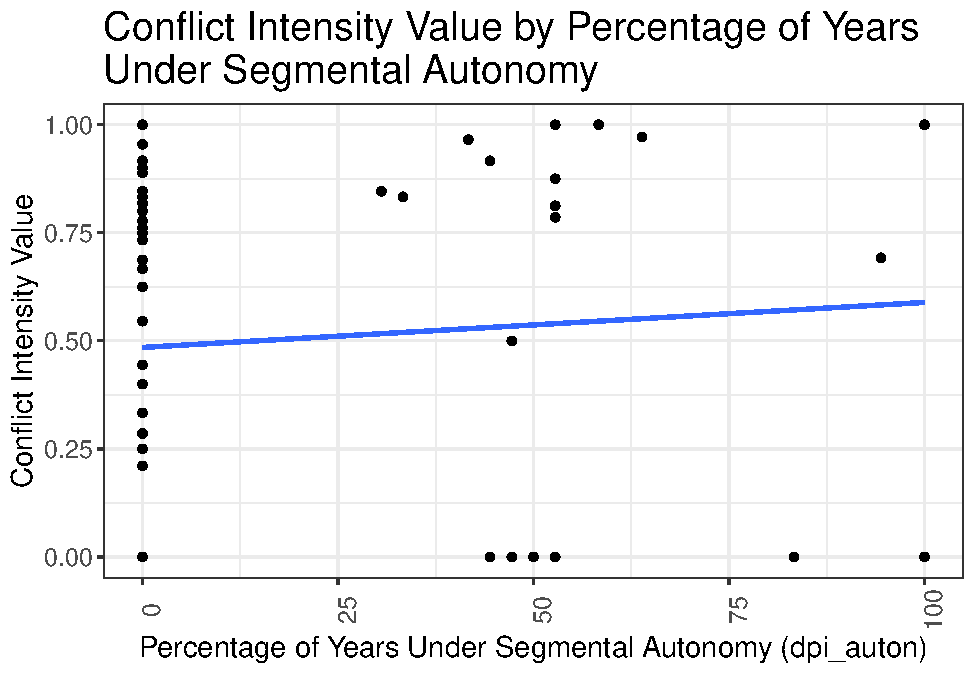
\includegraphics{03_tjbrailey_data_analysis_files/figure-latex/unnamed-chunk-2-1.pdf}

\hypertarget{qog-supportsatisfaction-with-democracy}{%
\subsection{QOG support/satisfaction with
democracy}\label{qog-supportsatisfaction-with-democracy}}

\begin{Shaded}
\begin{Highlighting}[]
\KeywordTok{csts}\NormalTok{(}\StringTok{"qog_hum_trust"}\NormalTok{, }\StringTok{"dpi_auton"}\NormalTok{)}
\end{Highlighting}
\end{Shaded}

\begin{verbatim}
## Joining, by = "country"
\end{verbatim}

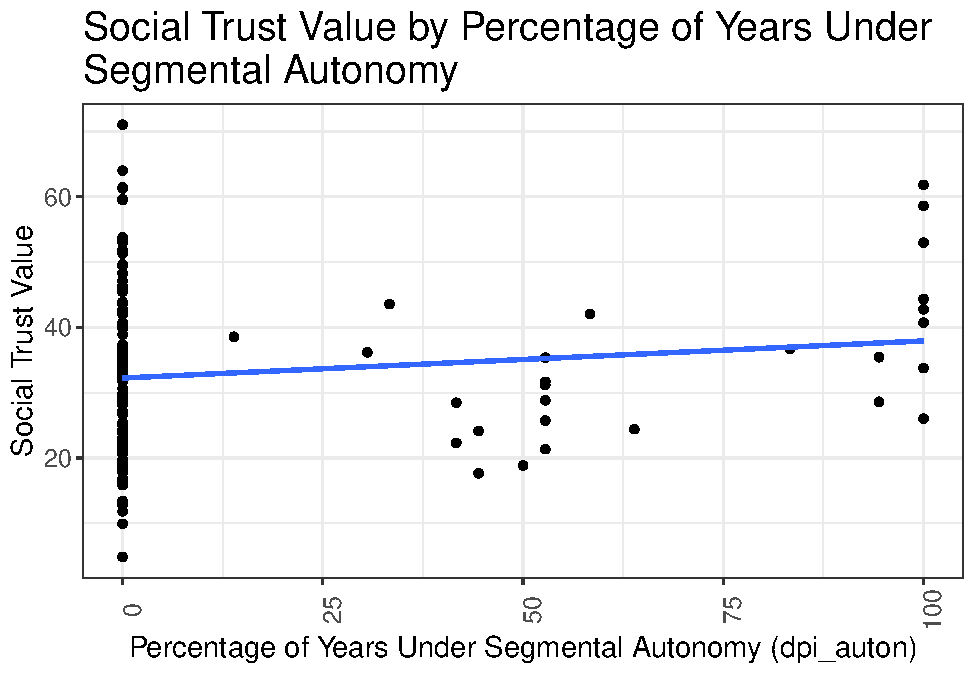
\includegraphics{03_tjbrailey_data_analysis_files/figure-latex/unnamed-chunk-3-1.pdf}

\begin{Shaded}
\begin{Highlighting}[]
\KeywordTok{csts}\NormalTok{(}\StringTok{"qog_hum_supdem"}\NormalTok{, }\StringTok{"dpi_auton"}\NormalTok{)}
\end{Highlighting}
\end{Shaded}

\begin{verbatim}
## Joining, by = "country"
\end{verbatim}

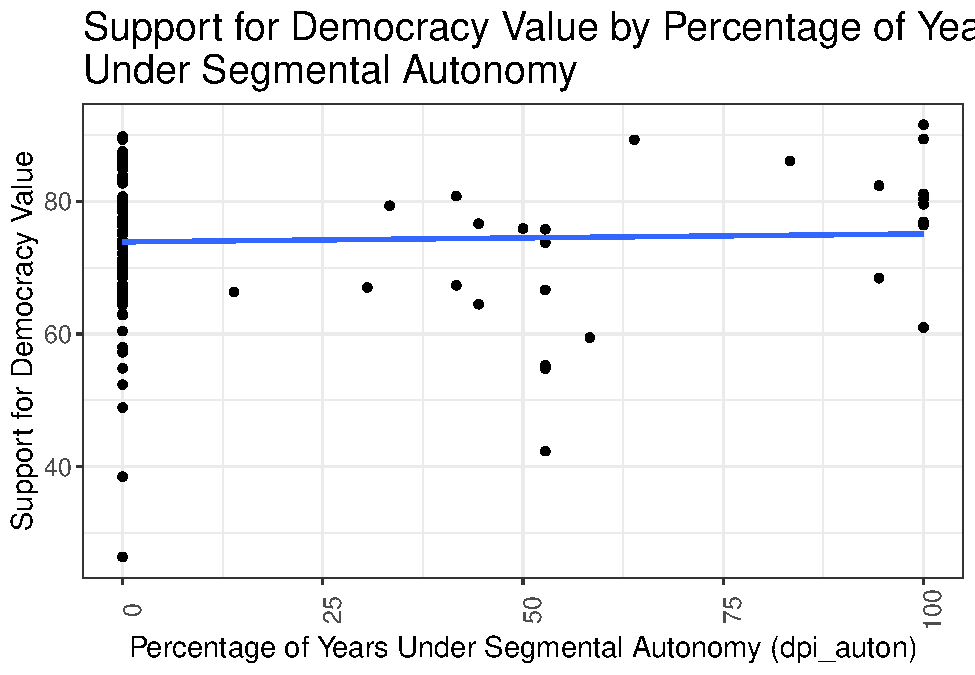
\includegraphics{03_tjbrailey_data_analysis_files/figure-latex/unnamed-chunk-3-2.pdf}

\begin{Shaded}
\begin{Highlighting}[]
\KeywordTok{csts}\NormalTok{(}\StringTok{"qog_hum_satdem"}\NormalTok{, }\StringTok{"dpi_auton"}\NormalTok{)}
\end{Highlighting}
\end{Shaded}

\begin{verbatim}
## Joining, by = "country"
\end{verbatim}

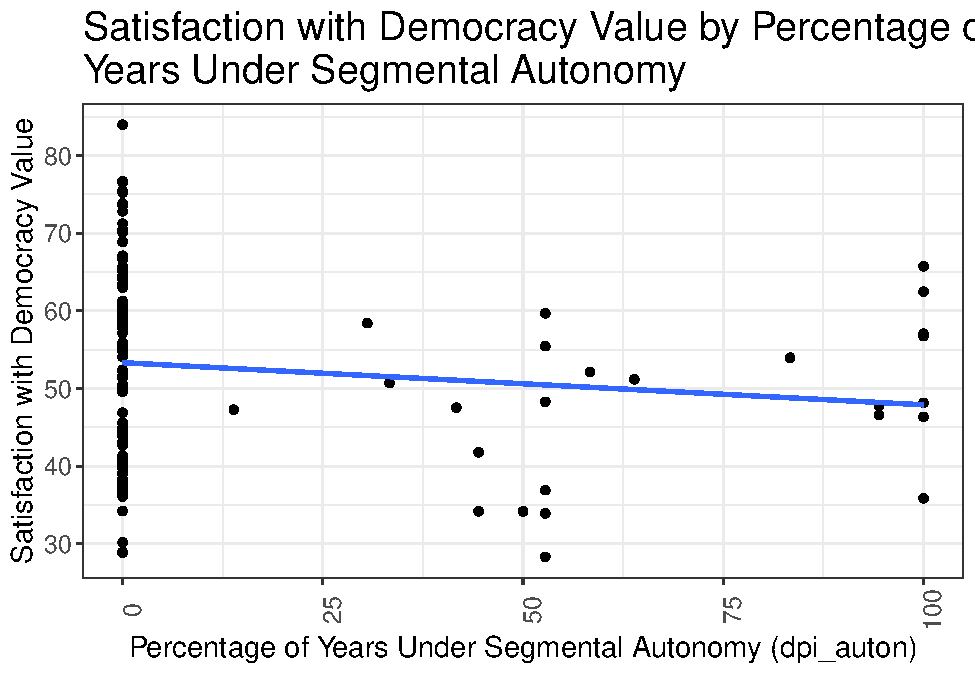
\includegraphics{03_tjbrailey_data_analysis_files/figure-latex/unnamed-chunk-3-3.pdf}

\hypertarget{polityiv-scores}{%
\subsection{PolityIV scores}\label{polityiv-scores}}

\begin{Shaded}
\begin{Highlighting}[]
\KeywordTok{csts}\NormalTok{(}\StringTok{"polity4_polity_score"}\NormalTok{, }\StringTok{"dpi_auton"}\NormalTok{)}
\end{Highlighting}
\end{Shaded}

\begin{verbatim}
## Joining, by = "country"
\end{verbatim}

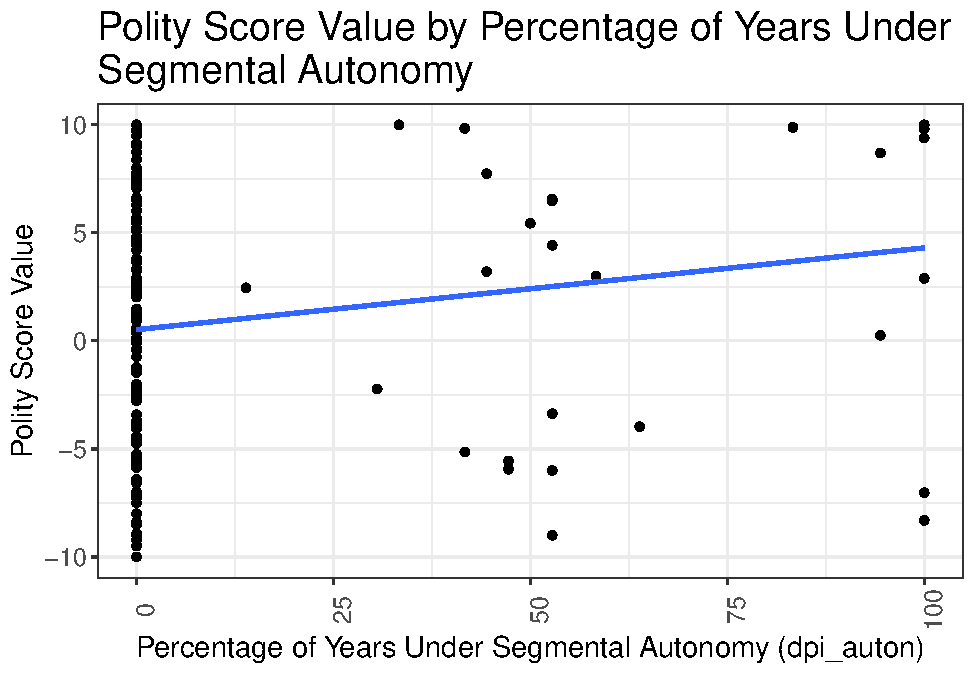
\includegraphics{03_tjbrailey_data_analysis_files/figure-latex/unnamed-chunk-4-1.pdf}

\hypertarget{linear-regressions}{%
\section{Linear regressions}\label{linear-regressions}}

\hypertarget{qog-supportsatisfaction-with-democracy-1}{%
\subsection{QOG support/satisfaction with
democracy}\label{qog-supportsatisfaction-with-democracy-1}}

\begin{Shaded}
\begin{Highlighting}[]
\KeywordTok{psp_lm}\NormalTok{(}\StringTok{"qog_hum_trust"}\NormalTok{, }\StringTok{"dpi_auton"}\NormalTok{)}
\end{Highlighting}
\end{Shaded}

\begin{verbatim}
## 1 coefficient  not defined because the design matrix is rank deficient
\end{verbatim}

\begin{verbatim}
## 2 coefficients  not defined because the design matrix is rank deficient
\end{verbatim}

\begin{verbatim}
## 1 coefficient  not defined because the design matrix is rank deficient
\end{verbatim}

\begin{verbatim}
## 2 coefficients  not defined because the design matrix is rank deficient
\end{verbatim}

\begin{verbatim}
## 
## \begin{table}
## \begin{center}
## \begin{tabular}{l c c c}
## \hline
##  & Model 1 & Model 2 & Model 3 \\
## \hline
## (Intercept)                  & $49.65^{***}$ & $22.38$   & $22.38$     \\
##                              & $(0.00)$      & $(12.09)$ & $(12.09)$   \\
## dpi\_auton                   & $0.40^{***}$  & $-30.83$  & $-30.83$    \\
##                              & $(0.00)$      & $(23.94)$ & $(23.94)$   \\
## qog\_wbgi\_pve               &               & $4.89$    & $4.89$      \\
##                              &               & $(5.03)$  & $(5.03)$    \\
## qog\_wdi\_gini               &               & $0.49$    & $0.49$      \\
##                              &               & $(0.32)$  & $(0.32)$    \\
## qog\_gle\_pop                &               & $0.00$    & $0.00$      \\
##                              &               & $(0.00)$  & $(0.00)$    \\
## polity4\_polity\_score       &               & $0.77$    & $0.77$      \\
##                              &               & $(0.82)$  & $(0.82)$    \\
## tb\_other\_provis            &               & $-12.28$  & $-12.28$    \\
##                              &               & $(3.39)$  & $(3.39)$    \\
## dpi\_auton:tb\_other\_provis &               &           & $29.00^{*}$ \\
##                              &               &           & $(5.98)$    \\
## \hline
## Country fixed effects        & $Y$           & $Y$       & $Y$         \\
## Year fixed effects           & $N$           & $Y$       & $Y$         \\
## R$^2$                        & $0.51$        & $0.58$    & $0.58$      \\
## Adj. R$^2$                   & $0.47$        & $0.51$    & $0.51$      \\
## Num. obs.                    & $598$         & $409$     & $409$       \\
## RMSE                         & $11.47$       & $11.53$   & $11.53$     \\
## \hline
## \multicolumn{4}{l}{\scriptsize{$^{***}p<0.001$; $^{**}p<0.01$; $^{*}p<0.05$}}
## \end{tabular}
## \caption{Statistical models}
## \label{table:coefficients}
## \end{center}
## \end{table}
\end{verbatim}

\begin{Shaded}
\begin{Highlighting}[]
\KeywordTok{psp_lm}\NormalTok{(}\StringTok{"qog_hum_trust"}\NormalTok{, }\StringTok{"epr_reg_aut_dum"}\NormalTok{)}
\end{Highlighting}
\end{Shaded}

\begin{verbatim}
## 1 coefficient  not defined because the design matrix is rank deficient
\end{verbatim}

\begin{verbatim}
## 1 coefficient  not defined because the design matrix is rank deficient
\end{verbatim}

\begin{verbatim}
## 
## \begin{table}
## \begin{center}
## \begin{tabular}{l c c c}
## \hline
##  & Model 1 & Model 2 & Model 3 \\
## \hline
## (Intercept)                          & $41.56^{**}$ & $22.95$   & $22.95$   \\
##                                      & $(0.36)$     & $(15.02)$ & $(15.02)$ \\
## epr\_reg\_aut\_dum                   & $8.09^{*}$   & $-3.26$   & $-32.21$  \\
##                                      & $(0.36)$     & $(8.19)$  & $(26.20)$ \\
## qog\_wbgi\_pve                       &              & $4.71$    & $4.71$    \\
##                                      &              & $(4.94)$  & $(4.94)$  \\
## qog\_wdi\_gini                       &              & $0.48$    & $0.48$    \\
##                                      &              & $(0.32)$  & $(0.32)$  \\
## qog\_gle\_pop                        &              & $0.00$    & $0.00$    \\
##                                      &              & $(0.00)$  & $(0.00)$  \\
## polity4\_polity\_score               &              & $0.67$    & $0.67$    \\
##                                      &              & $(0.79)$  & $(0.79)$  \\
## tb\_other\_provis                    &              & $-8.80$   & $-8.80$   \\
##                                      &              & $(4.45)$  & $(4.45)$  \\
## epr\_reg\_aut\_dum:tb\_other\_provis &              &           & $28.95$   \\
##                                      &              &           & $(24.03)$ \\
## \hline
## Country fixed effects                & $Y$          & $Y$       & $Y$       \\
## Year fixed effects                   & $N$          & $Y$       & $Y$       \\
## R$^2$                                & $0.52$       & $0.58$    & $0.58$    \\
## Adj. R$^2$                           & $0.48$       & $0.51$    & $0.51$    \\
## Num. obs.                            & $604$        & $415$     & $415$     \\
## RMSE                                 & $11.36$      & $11.48$   & $11.48$   \\
## \hline
## \multicolumn{4}{l}{\scriptsize{$^{***}p<0.001$; $^{**}p<0.01$; $^{*}p<0.05$}}
## \end{tabular}
## \caption{Statistical models}
## \label{table:coefficients}
## \end{center}
## \end{table}
\end{verbatim}

\begin{Shaded}
\begin{Highlighting}[]
\KeywordTok{psp_lm}\NormalTok{(}\StringTok{"qog_hum_trust"}\NormalTok{, }\StringTok{"rai_n_RAI"}\NormalTok{)}
\end{Highlighting}
\end{Shaded}

\begin{verbatim}
## 1 coefficient  not defined because the design matrix is rank deficient
\end{verbatim}

\begin{verbatim}
## 2 coefficients  not defined because the design matrix is rank deficient
\end{verbatim}

\begin{verbatim}
## 1 coefficient  not defined because the design matrix is rank deficient
\end{verbatim}

\begin{verbatim}
## 2 coefficients  not defined because the design matrix is rank deficient
\end{verbatim}

\begin{verbatim}
## 
## \begin{table}
## \begin{center}
## \begin{tabular}{l c c c}
## \hline
##  & Model 1 & Model 2 & Model 3 \\
## \hline
## (Intercept)                   & $-0.36$   & $69.00$   & $78.13^{*}$ \\
##                               & $(19.17)$ & $(28.16)$ & $(23.43)$   \\
## rai\_n\_RAI                   & $1.12$    & $-1.45$   & $-1.88$     \\
##                               & $(0.59)$  & $(0.73)$  & $(0.99)$    \\
## qog\_wbgi\_pve                &           & $2.98$    & $2.98$      \\
##                               &           & $(6.63)$  & $(6.63)$    \\
## qog\_wdi\_gini                &           & $-0.30$   & $-0.30$     \\
##                               &           & $(0.44)$  & $(0.44)$    \\
## qog\_gle\_pop                 &           & $-0.00$   & $-0.00$     \\
##                               &           & $(0.00)$  & $(0.00)$    \\
## polity4\_polity\_score        &           & $1.45$    & $1.45$      \\
##                               &           & $(1.37)$  & $(1.37)$    \\
## tb\_other\_provis             &           & $9.14$    &             \\
##                               &           & $(11.89)$ &             \\
## rai\_n\_RAI:tb\_other\_provis &           &           & $0.43$      \\
##                               &           &           & $(0.55)$    \\
## \hline
## Country fixed effects         & $Y$       & $Y$       & $Y$         \\
## Year fixed effects            & $N$       & $Y$       & $Y$         \\
## R$^2$                         & $0.62$    & $0.73$    & $0.73$      \\
## Adj. R$^2$                    & $0.60$    & $0.67$    & $0.67$      \\
## Num. obs.                     & $303$     & $194$     & $194$       \\
## RMSE                          & $10.51$   & $9.85$    & $9.85$      \\
## \hline
## \multicolumn{4}{l}{\scriptsize{$^{***}p<0.001$; $^{**}p<0.01$; $^{*}p<0.05$}}
## \end{tabular}
## \caption{Statistical models}
## \label{table:coefficients}
## \end{center}
## \end{table}
\end{verbatim}

\hypertarget{polityiv-scores-1}{%
\subsection{PolityIV scores}\label{polityiv-scores-1}}

\begin{Shaded}
\begin{Highlighting}[]
\CommentTok{# Polity score with DPI measurement of autonomy }
\KeywordTok{psp_lm}\NormalTok{(}\StringTok{"polity4_polity_score"}\NormalTok{, }\StringTok{"dpi_auton"}\NormalTok{)}
\end{Highlighting}
\end{Shaded}

\begin{verbatim}
## Warning in model.matrix.default(terms(formula, rhs = 1), data = mf): the
## response appeared on the right-hand side and was dropped
\end{verbatim}

\begin{verbatim}
## Warning in model.matrix.default(terms(formula, rhs = 1), data = mf): problem
## with term 7 in model.matrix: no columns are assigned
\end{verbatim}

\begin{verbatim}
## Warning in model.matrix.default(terms(formula, rhs = 1), data = mf): the
## response appeared on the right-hand side and was dropped
\end{verbatim}

\begin{verbatim}
## Warning in model.matrix.default(terms(formula, rhs = 1), data = mf): problem
## with term 8 in model.matrix: no columns are assigned
\end{verbatim}

\begin{verbatim}
## 1 coefficient  not defined because the design matrix is rank deficient
\end{verbatim}

\begin{verbatim}
## 2 coefficients  not defined because the design matrix is rank deficient
\end{verbatim}

\begin{verbatim}
## 1 coefficient  not defined because the design matrix is rank deficient
\end{verbatim}

\begin{verbatim}
## 2 coefficients  not defined because the design matrix is rank deficient
\end{verbatim}

\begin{verbatim}
## 
## \begin{table}
## \begin{center}
## \begin{tabular}{l c c c}
## \hline
##  & Model 1 & Model 2 & Model 3 \\
## \hline
## (Intercept)                  & $-7.27^{***}$ & $-4.07$  & $-4.07$       \\
##                              & $(0.00)$      & $(2.96)$ & $(2.96)$      \\
## dpi\_auton                   & $2.94$        & $0.24$   & $11.53^{***}$ \\
##                              & $(3.67)$      & $(1.55)$ & $(1.69)$      \\
## qog\_wbgi\_pve               &               & $0.87$   & $0.87$        \\
##                              &               & $(0.65)$ & $(0.65)$      \\
## qog\_wdi\_gini               &               & $0.02$   & $0.02$        \\
##                              &               & $(0.05)$ & $(0.05)$      \\
## qog\_gle\_pop                &               & $0.00$   & $0.00$        \\
##                              &               & $(0.00)$ & $(0.00)$      \\
## tb\_other\_provis            &               & $0.65$   & $0.65$        \\
##                              &               & $(0.77)$ & $(0.77)$      \\
## dpi\_auton:tb\_other\_provis &               &          & $-6.20^{*}$   \\
##                              &               &          & $(2.67)$      \\
## \hline
## Country fixed effects        & $Y$           & $Y$      & $Y$           \\
## Year fixed effects           & $N$           & $Y$      & $Y$           \\
## R$^2$                        & $0.64$        & $0.82$   & $0.82$        \\
## Adj. R$^2$                   & $0.63$        & $0.79$   & $0.79$        \\
## Num. obs.                    & $2379$        & $758$    & $758$         \\
## RMSE                         & $4.27$        & $2.35$   & $2.35$        \\
## \hline
## \multicolumn{4}{l}{\scriptsize{$^{***}p<0.001$; $^{**}p<0.01$; $^{*}p<0.05$}}
## \end{tabular}
## \caption{Statistical models}
## \label{table:coefficients}
## \end{center}
## \end{table}
\end{verbatim}

\begin{Shaded}
\begin{Highlighting}[]
\CommentTok{# Free and fair elections (robustness checks)}
\KeywordTok{psp_lm}\NormalTok{(}\StringTok{"v2elfrfair"}\NormalTok{, }\StringTok{"dpi_auton"}\NormalTok{)}
\end{Highlighting}
\end{Shaded}

\begin{verbatim}
## 1 coefficient  not defined because the design matrix is rank deficient
## 
## 2 coefficients  not defined because the design matrix is rank deficient
\end{verbatim}

\begin{verbatim}
## 1 coefficient  not defined because the design matrix is rank deficient
\end{verbatim}

\begin{verbatim}
## 2 coefficients  not defined because the design matrix is rank deficient
\end{verbatim}

\begin{verbatim}
## 
## \begin{table}
## \begin{center}
## \begin{tabular}{l c c c}
## \hline
##  & Model 1 & Model 2 & Model 3 \\
## \hline
## (Intercept)                  & $-1.39^{***}$ & $-0.64$     & $-0.64$      \\
##                              & $(0.00)$      & $(0.64)$    & $(0.64)$     \\
## dpi\_auton                   & $0.04$        & $-0.50$     & $1.80^{***}$ \\
##                              & $(1.56)$      & $(0.33)$    & $(0.36)$     \\
## qog\_wbgi\_pve               &               & $0.04$      & $0.04$       \\
##                              &               & $(0.08)$    & $(0.08)$     \\
## qog\_wdi\_gini               &               & $0.00$      & $0.00$       \\
##                              &               & $(0.01)$    & $(0.01)$     \\
## qog\_gle\_pop                &               & $-0.00$     & $-0.00$      \\
##                              &               & $(0.00)$    & $(0.00)$     \\
## polity4\_polity\_score       &               & $0.05^{**}$ & $0.05^{**}$  \\
##                              &               & $(0.01)$    & $(0.01)$     \\
## tb\_other\_provis            &               & $0.41^{*}$  & $0.41^{*}$   \\
##                              &               & $(0.15)$    & $(0.15)$     \\
## dpi\_auton:tb\_other\_provis &               &             & $-0.22$      \\
##                              &               &             & $(0.29)$     \\
## \hline
## Country fixed effects        & $Y$           & $Y$         & $Y$          \\
## Year fixed effects           & $N$           & $Y$         & $Y$          \\
## R$^2$                        & $0.69$        & $0.92$      & $0.92$       \\
## Adj. R$^2$                   & $0.68$        & $0.91$      & $0.91$       \\
## Num. obs.                    & $2111$        & $753$       & $753$        \\
## RMSE                         & $0.81$        & $0.36$      & $0.36$       \\
## \hline
## \multicolumn{4}{l}{\scriptsize{$^{***}p<0.001$; $^{**}p<0.01$; $^{*}p<0.05$}}
## \end{tabular}
## \caption{Statistical models}
## \label{table:coefficients}
## \end{center}
## \end{table}
\end{verbatim}

\begin{Shaded}
\begin{Highlighting}[]
\CommentTok{# Polity score with different measurements of regional autonomy (robustness checks)}
\KeywordTok{psp_lm}\NormalTok{(}\StringTok{"polity4_polity_score"}\NormalTok{, }\StringTok{"epr_reg_aut_dum"}\NormalTok{)}
\end{Highlighting}
\end{Shaded}

\begin{verbatim}
## Warning in model.matrix.default(terms(formula, rhs = 1), data = mf): the
## response appeared on the right-hand side and was dropped
\end{verbatim}

\begin{verbatim}
## Warning in model.matrix.default(terms(formula, rhs = 1), data = mf): problem
## with term 7 in model.matrix: no columns are assigned
\end{verbatim}

\begin{verbatim}
## Warning in model.matrix.default(terms(formula, rhs = 1), data = mf): the
## response appeared on the right-hand side and was dropped
\end{verbatim}

\begin{verbatim}
## Warning in model.matrix.default(terms(formula, rhs = 1), data = mf): problem
## with term 8 in model.matrix: no columns are assigned
\end{verbatim}

\begin{verbatim}
## 
## \begin{table}
## \begin{center}
## \begin{tabular}{l c c c}
## \hline
##  & Model 1 & Model 2 & Model 3 \\
## \hline
## (Intercept)                          & $-9.30^{***}$ & $-4.04$  & $-4.23$  \\
##                                      & $(1.16)$      & $(2.82)$ & $(2.86)$ \\
## epr\_reg\_aut\_dum                   & $2.79$        & $-1.24$  & $-0.25$  \\
##                                      & $(1.60)$      & $(1.41)$ & $(0.68)$ \\
## qog\_wbgi\_pve                       &               & $0.70$   & $0.71$   \\
##                                      &               & $(0.65)$ & $(0.65)$ \\
## qog\_wdi\_gini                       &               & $0.02$   & $0.02$   \\
##                                      &               & $(0.05)$ & $(0.05)$ \\
## qog\_gle\_pop                        &               & $0.00$   & $0.00$   \\
##                                      &               & $(0.00)$ & $(0.00)$ \\
## tb\_other\_provis                    &               & $0.07$   & $0.07$   \\
##                                      &               & $(0.70)$ & $(0.70)$ \\
## epr\_reg\_aut\_dum:tb\_other\_provis &               &          & $-1.55$  \\
##                                      &               &          & $(2.11)$ \\
## \hline
## Country fixed effects                & $Y$           & $Y$      & $Y$      \\
## Year fixed effects                   & $N$           & $Y$      & $Y$      \\
## R$^2$                                & $0.64$        & $0.81$   & $0.81$   \\
## Adj. R$^2$                           & $0.63$        & $0.79$   & $0.79$   \\
## Num. obs.                            & $2410$        & $773$    & $773$    \\
## RMSE                                 & $4.25$        & $2.38$   & $2.38$   \\
## \hline
## \multicolumn{4}{l}{\scriptsize{$^{***}p<0.001$; $^{**}p<0.01$; $^{*}p<0.05$}}
## \end{tabular}
## \caption{Statistical models}
## \label{table:coefficients}
## \end{center}
## \end{table}
\end{verbatim}

\begin{Shaded}
\begin{Highlighting}[]
\KeywordTok{psp_lm}\NormalTok{(}\StringTok{"polity4_polity_score"}\NormalTok{, }\StringTok{"rai_n_RAI"}\NormalTok{)}
\end{Highlighting}
\end{Shaded}

\begin{verbatim}
## Warning in model.matrix.default(terms(formula, rhs = 1), data = mf): the
## response appeared on the right-hand side and was dropped
\end{verbatim}

\begin{verbatim}
## Warning in model.matrix.default(terms(formula, rhs = 1), data = mf): problem
## with term 7 in model.matrix: no columns are assigned
\end{verbatim}

\begin{verbatim}
## Warning in model.matrix.default(terms(formula, rhs = 1), data = mf): the
## response appeared on the right-hand side and was dropped
\end{verbatim}

\begin{verbatim}
## Warning in model.matrix.default(terms(formula, rhs = 1), data = mf): problem
## with term 8 in model.matrix: no columns are assigned
\end{verbatim}

\begin{verbatim}
## 1 coefficient  not defined because the design matrix is rank deficient
\end{verbatim}

\begin{verbatim}
## 1 coefficient  not defined because the design matrix is rank deficient
## 
## 1 coefficient  not defined because the design matrix is rank deficient
## 
## 1 coefficient  not defined because the design matrix is rank deficient
\end{verbatim}

\begin{verbatim}
## 
## \begin{table}
## \begin{center}
## \begin{tabular}{l c c c}
## \hline
##  & Model 1 & Model 2 & Model 3 \\
## \hline
## (Intercept)                   & $-22.59^{**}$ &          &          \\
##                               & $(4.69)$      &          &          \\
## rai\_n\_RAI                   & $1.03^{**}$   & $0.41$   & $-8.19$  \\
##                               & $(0.15)$      & $(0.29)$ & $(8.35)$ \\
## qog\_wbgi\_pve                &               & $0.36$   & $0.33$   \\
##                               &               & $(0.46)$ & $(0.48)$ \\
## qog\_wdi\_gini                &               & $-0.06$  & $-0.06$  \\
##                               &               & $(0.07)$ & $(0.07)$ \\
## qog\_gle\_pop                 &               & $0.00$   & $0.00$   \\
##                               &               & $(0.00)$ & $(0.00)$ \\
## tb\_other\_provis             &               & $-3.83$  & $-3.94$  \\
##                               &               & $(8.34)$ & $(8.35)$ \\
## rai\_n\_RAI:tb\_other\_provis &               &          & $8.60$   \\
##                               &               &          & $(8.25)$ \\
## \hline
## Country fixed effects         & $Y$           & $Y$      & $Y$      \\
## Year fixed effects            & $N$           & $Y$      & $Y$      \\
## R$^2$                         & $0.66$        & $0.77$   & $0.77$   \\
## Adj. R$^2$                    & $0.65$        & $0.73$   & $0.73$   \\
## Num. obs.                     & $594$         & $221$    & $221$    \\
## RMSE                          & $3.11$        & $1.03$   & $1.03$   \\
## \hline
## \multicolumn{4}{l}{\scriptsize{$^{***}p<0.001$; $^{**}p<0.01$; $^{*}p<0.05$}}
## \end{tabular}
## \caption{Statistical models}
## \label{table:coefficients}
## \end{center}
## \end{table}
\end{verbatim}

\hypertarget{cox-regressions}{%
\section{Cox regressions}\label{cox-regressions}}

\begin{Shaded}
\begin{Highlighting}[]
\CommentTok{# DPI}
\NormalTok{cox1 <-}\StringTok{ }\NormalTok{survival}\OperatorTok{::}\KeywordTok{coxph}\NormalTok{(survival}\OperatorTok{::}\KeywordTok{Surv}\NormalTok{(year, ucdp_cumulative_intensity) }\OperatorTok{~}\StringTok{ }\NormalTok{(dpi_auton }\OperatorTok{*}\StringTok{ }\NormalTok{tb_other_provis) }\OperatorTok{+}\StringTok{ }\NormalTok{qog_wbgi_pve }\OperatorTok{+}\StringTok{ }\NormalTok{qog_wdi_gini }\OperatorTok{+}\StringTok{ }\NormalTok{qog_gle_pop }\OperatorTok{+}\StringTok{ }\NormalTok{polity4_polity_score, }\DataTypeTok{data =}\NormalTok{ psp)}
\CommentTok{#summary(cox1)}
\CommentTok{#reporttools::displayCoxPH(cox1)}

\CommentTok{# EPR}
\NormalTok{cox2 <-}\StringTok{ }\NormalTok{survival}\OperatorTok{::}\KeywordTok{coxph}\NormalTok{(survival}\OperatorTok{::}\KeywordTok{Surv}\NormalTok{(year, ucdp_cumulative_intensity) }\OperatorTok{~}\StringTok{ }\NormalTok{(epr_reg_aut_dum }\OperatorTok{*}\StringTok{ }\NormalTok{tb_other_provis) }\OperatorTok{+}\StringTok{ }\KeywordTok{as.factor}\NormalTok{(country) }\OperatorTok{+}\StringTok{ }\NormalTok{qog_wbgi_pve }\OperatorTok{+}\StringTok{ }\NormalTok{qog_wdi_gini }\OperatorTok{+}\StringTok{ }\NormalTok{qog_gle_pop }\OperatorTok{+}\StringTok{ }\NormalTok{polity4_polity_score, }\DataTypeTok{data =}\NormalTok{ psp)}
\end{Highlighting}
\end{Shaded}

\begin{verbatim}
## Warning in fitter(X, Y, istrat, offset, init, control, weights = weights, :
## Loglik converged before variable 13,32,35,50,62,68,102,104,106,118,119,123,172 ;
## coefficient may be infinite.
\end{verbatim}

\begin{Shaded}
\begin{Highlighting}[]
\CommentTok{#summary(cox2)}
\CommentTok{#reporttools::displayCoxPH(cox2)}

\CommentTok{# RAI}
\NormalTok{cox3 <-}\StringTok{ }\NormalTok{survival}\OperatorTok{::}\KeywordTok{coxph}\NormalTok{(survival}\OperatorTok{::}\KeywordTok{Surv}\NormalTok{(year, ucdp_cumulative_intensity) }\OperatorTok{~}\StringTok{ }\NormalTok{(rai_n_RAI }\OperatorTok{*}\StringTok{ }\NormalTok{tb_other_provis) }\OperatorTok{+}\StringTok{ }\KeywordTok{as.factor}\NormalTok{(country) }\OperatorTok{+}\StringTok{ }\NormalTok{qog_wbgi_pve }\OperatorTok{+}\StringTok{ }\NormalTok{qog_wdi_gini }\OperatorTok{+}\StringTok{ }\NormalTok{qog_gle_pop }\OperatorTok{+}\StringTok{ }\NormalTok{polity4_polity_score, }\DataTypeTok{data =}\NormalTok{ psp)}
\end{Highlighting}
\end{Shaded}

\begin{verbatim}
## Warning in fitter(X, Y, istrat, offset, init, control, weights = weights, :
## Loglik converged before variable 1,2,106,159,189 ; coefficient may be infinite.
\end{verbatim}

\begin{Shaded}
\begin{Highlighting}[]
\CommentTok{#summary(cox3)}
\CommentTok{#reporttools::displayCoxPH(cox3)}
\end{Highlighting}
\end{Shaded}

\hypertarget{multivariate-comparison-across-operationalizations}{%
\section{Multivariate comparison across
operationalizations}\label{multivariate-comparison-across-operationalizations}}

\begin{Shaded}
\begin{Highlighting}[]
\NormalTok{psp <-}\StringTok{ }\NormalTok{psp }\OperatorTok
\StringTok{    }\NormalTok{dplyr}\OperatorTok{::}\KeywordTok{mutate_if}\NormalTok{(is.numeric, round, }\DataTypeTok{digits =} \DecValTok{3}\NormalTok{) }\OperatorTok
\StringTok{    }\NormalTok{dplyr}\OperatorTok{::}\KeywordTok{filter}\NormalTok{(qog_fe_etfra }\OperatorTok{>}\StringTok{ }\KeywordTok{median}\NormalTok{(psp}\OperatorTok{$}\NormalTok{qog_fe_etfra, }\DataTypeTok{na.rm =} \OtherTok{TRUE}\NormalTok{))}

\NormalTok{dpi_reg <-}\StringTok{ }\NormalTok{estimatr}\OperatorTok{::}\KeywordTok{lm_robust}\NormalTok{(polity4_polity_score }\OperatorTok{~}\StringTok{ }\NormalTok{(dpi_auton }\OperatorTok{*}\StringTok{ }\NormalTok{tb_other_provis) }\OperatorTok{+}\StringTok{ }\KeywordTok{as.factor}\NormalTok{(country) }\OperatorTok{+}\StringTok{ }\KeywordTok{as.factor}\NormalTok{(year) }\OperatorTok{+}\StringTok{ }\NormalTok{qog_wbgi_pve }\OperatorTok{+}\StringTok{ }\NormalTok{qog_wdi_gini }\OperatorTok{+}\StringTok{ }\NormalTok{qog_gle_pop, }\DataTypeTok{data =}\NormalTok{ psp, }\DataTypeTok{se_type =} \StringTok{"CR2"}\NormalTok{, }\DataTypeTok{clusters =}\NormalTok{ country)}

\NormalTok{epr_reg <-}\StringTok{ }\NormalTok{estimatr}\OperatorTok{::}\KeywordTok{lm_robust}\NormalTok{(polity4_polity_score }\OperatorTok{~}\StringTok{ }\NormalTok{(epr_reg_aut_dum }\OperatorTok{*}\StringTok{ }\NormalTok{tb_other_provis) }\OperatorTok{+}\StringTok{ }\KeywordTok{as.factor}\NormalTok{(country) }\OperatorTok{+}\StringTok{ }\KeywordTok{as.factor}\NormalTok{(year) }\OperatorTok{+}\StringTok{ }\NormalTok{qog_wbgi_pve }\OperatorTok{+}\StringTok{ }\NormalTok{qog_wdi_gini }\OperatorTok{+}\StringTok{ }\NormalTok{qog_gle_pop, }\DataTypeTok{data =}\NormalTok{ psp, }\DataTypeTok{se_type =} \StringTok{"CR2"}\NormalTok{, }\DataTypeTok{clusters =}\NormalTok{ country)}

\NormalTok{rai_reg <-}\StringTok{ }\NormalTok{estimatr}\OperatorTok{::}\KeywordTok{lm_robust}\NormalTok{(polity4_polity_score }\OperatorTok{~}\StringTok{ }\NormalTok{(rai_n_RAI }\OperatorTok{*}\StringTok{ }\NormalTok{tb_other_provis) }\OperatorTok{+}\StringTok{ }\KeywordTok{as.factor}\NormalTok{(country) }\OperatorTok{+}\StringTok{ }\KeywordTok{as.factor}\NormalTok{(year) }\OperatorTok{+}\StringTok{ }\NormalTok{qog_wbgi_pve }\OperatorTok{+}\StringTok{ }\NormalTok{qog_wdi_gini }\OperatorTok{+}\StringTok{ }\NormalTok{qog_gle_pop, }\DataTypeTok{data =}\NormalTok{ psp, }\DataTypeTok{se_type =} \StringTok{"CR2"}\NormalTok{, }\DataTypeTok{clusters =}\NormalTok{ country)}

\NormalTok{tex_fin <-}\StringTok{ }\NormalTok{texreg}\OperatorTok{::}\KeywordTok{texreg}\NormalTok{(}\KeywordTok{list}\NormalTok{(dpi_reg, epr_reg, rai_reg), }\DataTypeTok{mfrow =} \OtherTok{TRUE}\NormalTok{, }
                                \DataTypeTok{omit.coef =} \StringTok{"as.factor"}\NormalTok{, }
                                \DataTypeTok{include.ci =} \OtherTok{FALSE}\NormalTok{, }
                                \DataTypeTok{custom.gof.rows =} \KeywordTok{list}\NormalTok{(}\StringTok{`}\DataTypeTok{Country fixed effects}\StringTok{`}\NormalTok{ =}\StringTok{ }\KeywordTok{c}\NormalTok{(}\StringTok{"Y"}\NormalTok{, }\StringTok{"Y"}\NormalTok{, }\StringTok{"Y"}\NormalTok{),}
                                                       \StringTok{`}\DataTypeTok{Year fixed effects}\StringTok{`}\NormalTok{ =}\StringTok{ }\KeywordTok{c}\NormalTok{(}\StringTok{"Y"}\NormalTok{, }\StringTok{"Y"}\NormalTok{, }\StringTok{"Y"}\NormalTok{)))}
\end{Highlighting}
\end{Shaded}

\begin{verbatim}
## 2 coefficients  not defined because the design matrix is rank deficient
\end{verbatim}

\begin{verbatim}
## 1 coefficient  not defined because the design matrix is rank deficient
\end{verbatim}

\begin{Shaded}
\begin{Highlighting}[]
\NormalTok{tex_fin}
\end{Highlighting}
\end{Shaded}

\begin{verbatim}
## 
## \begin{table}
## \begin{center}
## \begin{tabular}{l c c c}
## \hline
##  & Model 1 & Model 2 & Model 3 \\
## \hline
## (Intercept)                          & $-4.07$       & $-4.23$  &          \\
##                                      & $(2.96)$      & $(2.86)$ &          \\
## dpi\_auton                           & $11.53^{***}$ &          &          \\
##                                      & $(1.69)$      &          &          \\
## tb\_other\_provis                    & $0.65$        & $0.07$   & $-3.94$  \\
##                                      & $(0.77)$      & $(0.70)$ & $(8.35)$ \\
## qog\_wbgi\_pve                       & $0.87$        & $0.71$   & $0.33$   \\
##                                      & $(0.65)$      & $(0.65)$ & $(0.48)$ \\
## qog\_wdi\_gini                       & $0.02$        & $0.02$   & $-0.06$  \\
##                                      & $(0.05)$      & $(0.05)$ & $(0.07)$ \\
## qog\_gle\_pop                        & $0.00$        & $0.00$   & $0.00$   \\
##                                      & $(0.00)$      & $(0.00)$ & $(0.00)$ \\
## dpi\_auton:tb\_other\_provis         & $-6.20^{*}$   &          &          \\
##                                      & $(2.67)$      &          &          \\
## epr\_reg\_aut\_dum                   &               & $-0.25$  &          \\
##                                      &               & $(0.68)$ &          \\
## epr\_reg\_aut\_dum:tb\_other\_provis &               & $-1.55$  &          \\
##                                      &               & $(2.11)$ &          \\
## rai\_n\_RAI                          &               &          & $-8.19$  \\
##                                      &               &          & $(8.35)$ \\
## rai\_n\_RAI:tb\_other\_provis        &               &          & $8.60$   \\
##                                      &               &          & $(8.25)$ \\
## \hline
## Country fixed effects                & $Y$           & $Y$      & $Y$      \\
## Year fixed effects                   & $Y$           & $Y$      & $Y$      \\
## R$^2$                                & $0.82$        & $0.81$   & $0.77$   \\
## Adj. R$^2$                           & $0.79$        & $0.79$   & $0.73$   \\
## Num. obs.                            & $758$         & $773$    & $221$    \\
## RMSE                                 & $2.35$        & $2.38$   & $1.03$   \\
## \hline
## \multicolumn{4}{l}{\scriptsize{$^{***}p<0.001$; $^{**}p<0.01$; $^{*}p<0.05$}}
## \end{tabular}
## \caption{Statistical models}
## \label{table:coefficients}
## \end{center}
## \end{table}
\end{verbatim}

\end{document}
